
\section{Summary}

In this thesis, we examined degradation bias in long-read direct RNA-seq. We first characterised degradation by formalising the notion of the degradation rate, and estimated degradation rates across different human cell lines. We showed that degradation rates are consistent across isoforms and their features. By examining degradation in sequencing spike-ins, we find that degradation in endogenous RNA is likely to be a combination of \textit{in vivo} RNA decay and extraneous \textit{in vitro} factors. Next, we developed a bias-aware model for transcript quantification that models the probability of observing a read originating from an isoform based on a read length-isoform agreement model. We derive an expectation maximization algorithm for inferring degradation-aware isoform abundance estimates. To evaluate our model, we perform benchmarking against existing methods for transcript quantification. On simulated datasets with known degradation, our model outperforms other methods on both reference and subset isoforms. On real datasets with sequencing spike-ins, our model achieves results of comparable accuracy to those of existing methods and admits greater reproducibility. 

\section{Further work}

To conclude, we highlight four areas of future work.

\subsection{Gene-specific degradation}

Currently, our bias model fits the degradation rate per base globally, with the assumption that the degradation rate per base is the same across all isoforms. The validity of this assumption depends on the source of the degradation - if the degradation is mostly a product of RNA decay \textit{in vivo}, then this assumption is unlikely to hold, since differential rates of RNA decay have been extensively described. However, if the degradation is mostly an artifact of the library preparation or sequencing, then a global degradation rate may apply across the isoforms. Nevertheless, it might still be of interest to fit \textit{gene-level degradation rates}, as this would likely improve the accuracy of abundance estimates and reflect the underlying biology more faithfully. 

\subsection{Unobserved degradation for short isoforms}

While we characterised degradation from the data via the read length distribution of the \textit{observed} degraded reads, it is possible that through the entire process of sequencing, transcripts or reads from shorter isoforms would have been fully degraded. This would lead to an underestimation of the counts for short isoforms, and possibly warrant some form of length normalisation for the data. Developing experiments to examine degradation over the course of a sequencing experiment for modeling \textit{unobserved degraded reads} is one potential area of future work.  

\subsection{Novel isoform discovery}

One attractive benefit of longer reads from ONT sequencing is the potential to discover and characterise novel isoforms. Currently, our model admits transcriptome alignments and does not perform discovery. It is possible to couple our model with a tool capable of transcript discovery, such as Bambu, by first producing extended transcriptome annotations with transcript discovery, and running our model for bias-aware transcript quantification.  

\subsection{Read position-isoform agreement}

To model bias, we introduced the read length-isoform agreement, which models the probability of observing a read of a certain length originating from an isoform and its degradation rate. Our current model applies however only to direct RNA-seq, as we assume that the 3' end of all reads align within a close proximity to the annotated 3' end of the isoform. However, it is well known that annotations at both the 5' and 3' end are not clearly well-defined and unreliable. In addition, for direct cDNA and PCR-cDNA protocols, a fraction of reads may not align at the 3' end, resulting in an underestimation of the count. To mitigate these issues and generalise our model to cDNA protocols, we can consider a \textit{read position-isoform agreement} that models the probability of observing a read at a certain start/end position within the sequence of an isoform. 

\begin{figure}
    \centering
    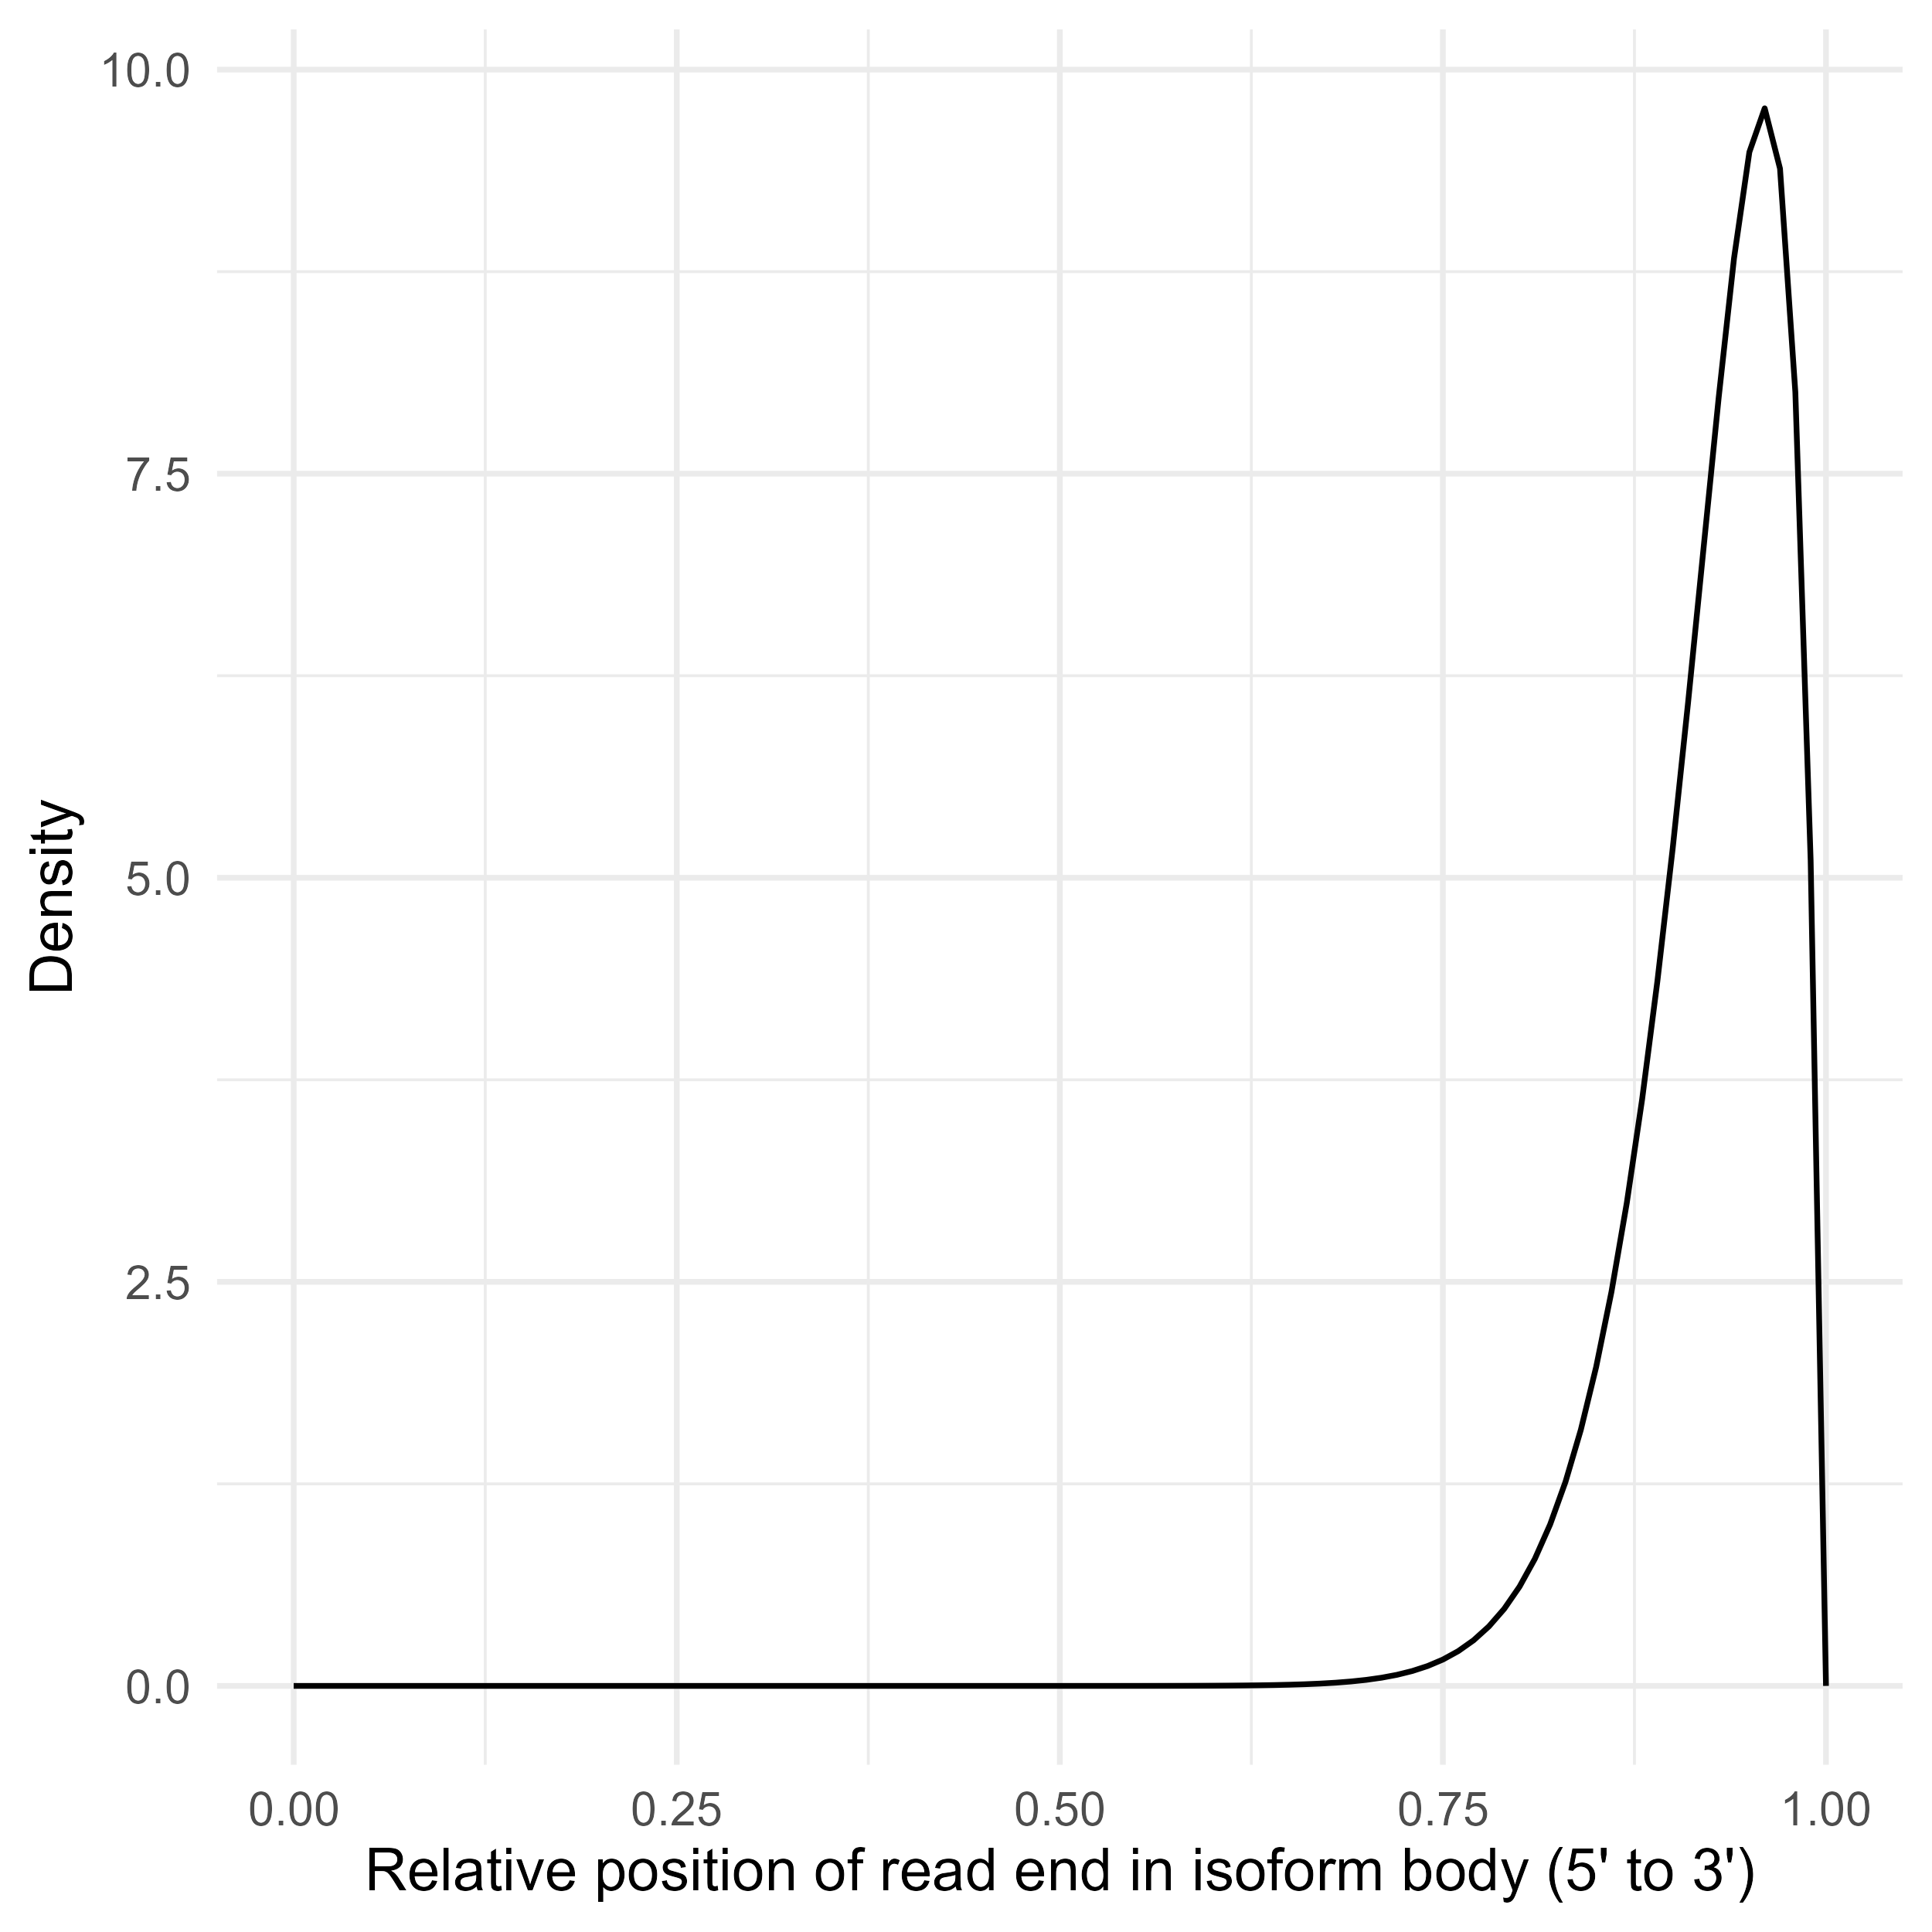
\includegraphics{figures/position}
    \caption{Caption}
    \label{fig:my_label}
\end{figure}
